%!TEX TS-program = xelatex

% Официальный шаблон презентации НИУ ВШЭ в beamer (LaTeX)
% Версия 2.0
% Язык — русский   
% Автор шаблона - Данил Фёдоровых (fedorovykh@gmail.com)

%%% Для корректной работы шаблона необходима 
%%% установка в систему бесплатного шрифта HSE Sans
%%% https://www.hse.ru/info/brandbook/#font


\documentclass[aspectratio=169]{beamer}

\usepackage{HSE-theme/beamerthemeHSE} % Подгружаем тему

%%% Работа с русским языком и шрифтами
\usepackage[english,russian]{babel}   % загружает пакет многоязыковой вёрстки
\usepackage{fontspec}      % подготавливает загрузку шрифтов Open Type, True Type и др.
\setsansfont{HSE Sans} 
\setmonofont{Courier New}
% \setmainfont{Arial}
% \setsansfont{Arial}
\uselanguage{russian}
\languagepath{russian}
\deftranslation[to=russian]{Theorem}{Теорема}
\deftranslation[to=russian]{Definition}{Определение}
\deftranslation[to=russian]{Definitions}{Определения}
\deftranslation[to=russian]{Corollary}{Следствие}
\deftranslation[to=russian]{Fact}{Факт}
\deftranslation[to=russian]{Example}{Пример}
\deftranslation[to=russian]{Examples}{Примеры}

%multi-row
\usepackage{multirow}
\usepackage{caption}
\usepackage{amssymb}% http://ctan.org/pkg/amssymb
\usepackage{pifont}% http://ctan.org/pkg/pifont
\usepackage{blindtext} 		% Случайный текст
\graphicspath{{images/}}  	% Папка с картинками

%%% Информация об авторе и выступлении
\title[Заголовок]{Колоризация изображений} 
%\subtitle{}
\author{Головин Вячеслав \and Саленек Иван}
%\institute{Название подразделения одну, две или три строки}
\date{\today}

\begin{document}	% Начало презентации
\renewcommand{\inserttotalframenumber}{8}   % Надо будет починить

\frame[plain]{\titlepage}	% Титульный слайд

\begin{frame}{Постановка задачи}
%\framesubtitle{}
\begin{columns}
    \begin{column}{.6\textwidth}
    \begin{itemize}
        \item Колоризация черно-белых изображений при помощи нейронныых сетей
        
        \item Обзор существующих решений и попытка их улучшения
    \end{itemize}
    \end{column}
    \begin{column}{.4\textwidth}
    \begin{figure}
        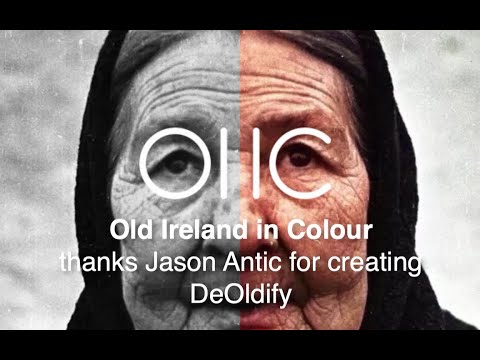
\includegraphics[width=\textwidth]{DeOldify.jpeg}
        \caption*{Проект DeOldify}
    \end{figure}
    \end{column}
\end{columns}



\end{frame}

\begin{frame}{\href{https://github.com/richzhang/colorization}{Colorful Image Colorization} (2016, 2017)}
\framesubtitle{Известные результаты}
        \begin{figure}
            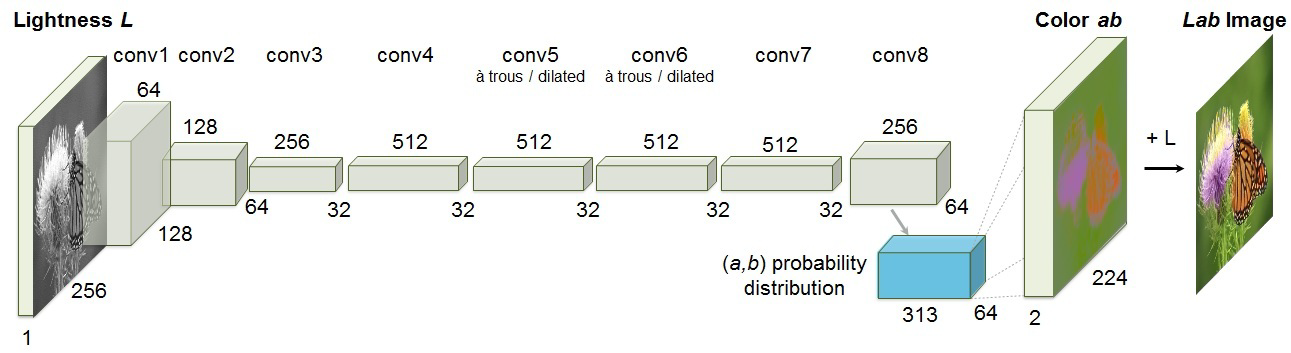
\includegraphics[width=0.6\textwidth]{eccv16.png}
            \caption*{ECCV16}
        \end{figure}

        \begin{figure}
            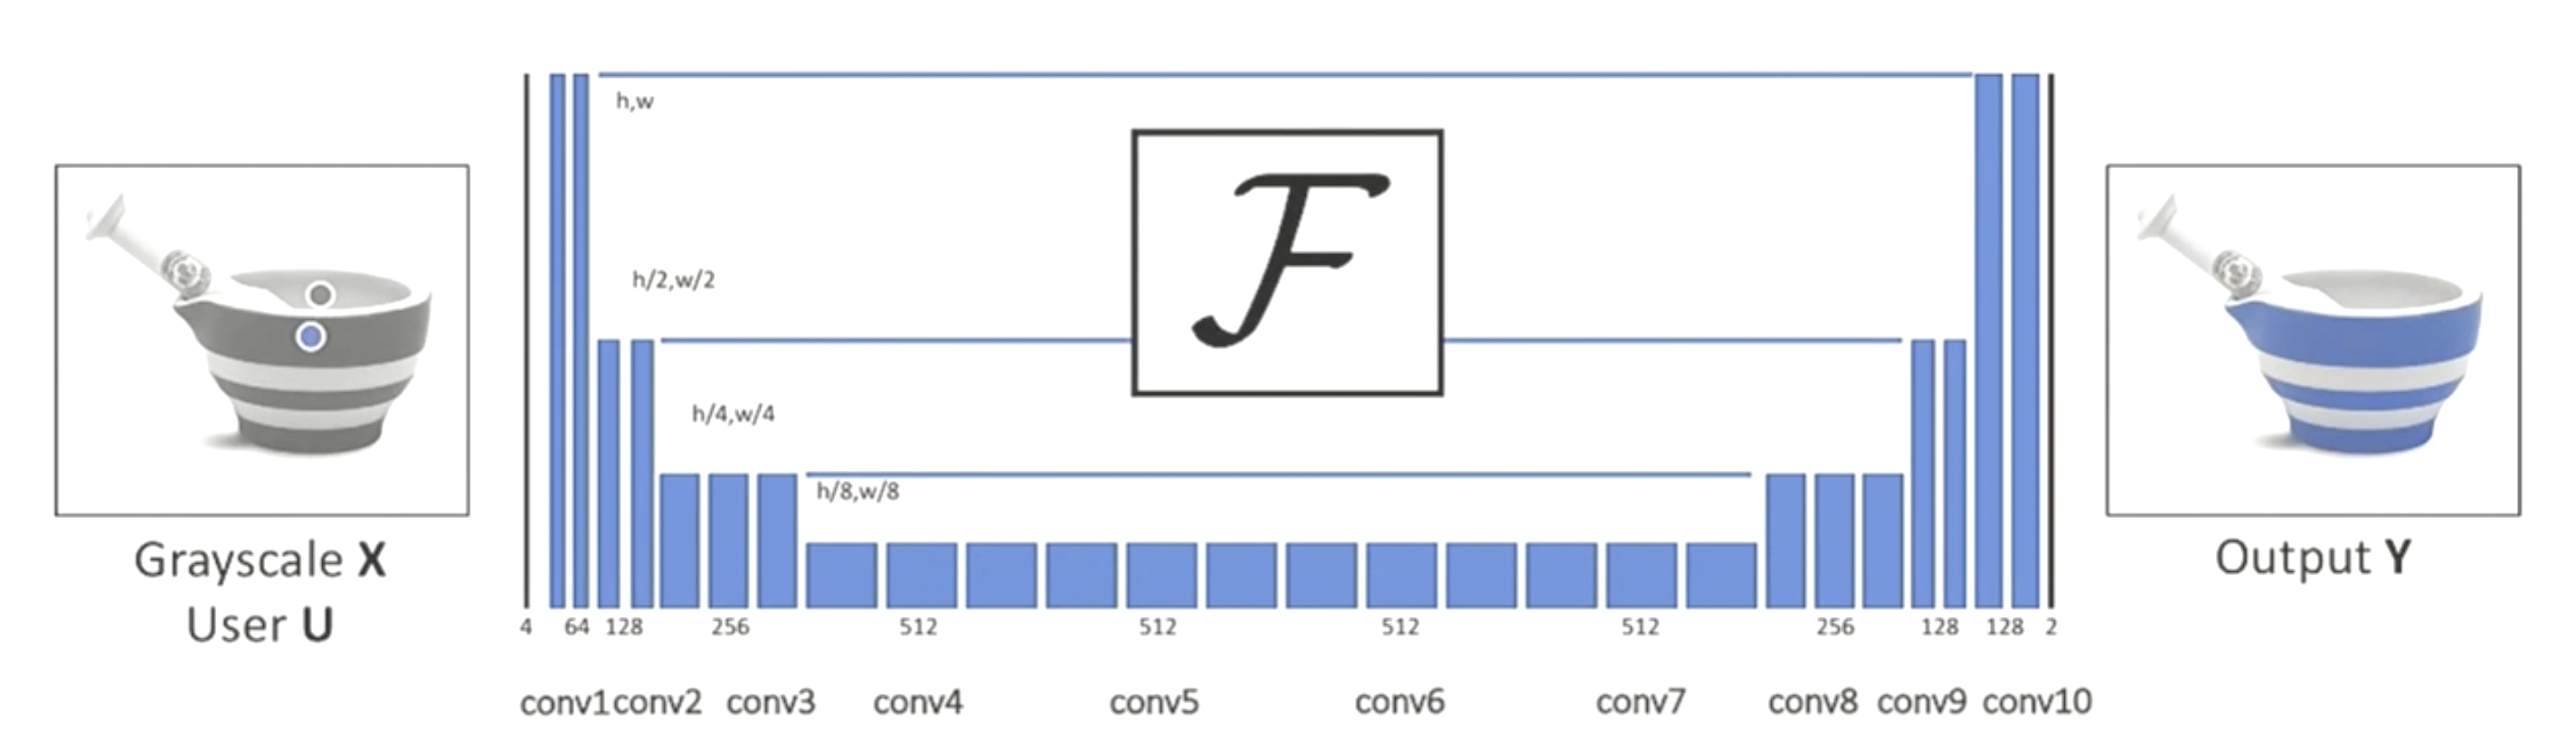
\includegraphics[width=0.6\textwidth]{siggraph17_white.png}
            \caption*{Siggraph17}
        \end{figure}
\end{frame}

\begin{frame}{\href{https://github.com/jantic/DeOldify}{DeOldify} (2018)}
    \framesubtitle{Известные результаты}

    В основе \textbf{DeOldify} лежит \textbf{GAN} архитектура. Автор использует собственный \textbf{NoGAN} подход, для обучения генератора и критика\\[3mm]
    
    Генераторам выступает \textbf{U-Net} из фреймворка \texttt{fast.ai}, позволяющего использовать предобученную сеть (н-р \textbf{ResNet}) в качестве основы для \textbf{U-Net}\\[3mm]

    \textbf{DeOldify} предлагает \textbf{2} предобученных "колорайзера":\\[3mm]
    \begin{itemize}
        \item \textbf{Artistic} -- \texttt{resnet34} в основе \textbf{U-Net} + 5 \textbf{NoGAN} итераций. \\
        $\checkmark$ Более яркие и детальные результаты \\
        \ding{55} {} Возникают артефакты
        \item \textbf{Stable} -- \texttt{resnet101} в основе \textbf{U-Net} + 3 \textbf{NoGAN} итерации. \\ 
        $\checkmark$ Лучше работает для пейзажей и портретов \\
        \ding{55} {} Более тусклые цвета
    \end{itemize}
\end{frame}

\begin{frame}{Реализованные бейзлайны}
%\framesubtitle{}
\begin{itemize}
\item В качестве базовых метрик были взяты \textbf{Feature Loss}, основанный на \textbf{VGG16}, и обычный \textbf{MSE}.
    \item Метрики были посчитаны для \textbf{1000} "колоризованых"\ картинок из \textbf{ImageNet} (\href{https://drive.google.com/drive/folders/1ebPVAsKlLlXY2Tg8Q1TXbiTRhfdegI40}{ссылка на папку с результатами})
\end{itemize}

\begin{table}\bf
    \begin{tabular}{l|c|c|c|c}
    \hline
    \multicolumn{5}{c}{Colorization Results on 1000 224x224 images}\\ 
    \hline
    \hline
    \multirow{3}{*}{Method} & \multicolumn{2}{c|}{Model} &  \multicolumn{2}{c}{Losses}\\
                            & Params & Runtime & VGG16 & MSE \\
                            & (MB) & (s) & (loss) & (loss) \\
    \hline
    CIC-ECCV16 & 129 & 250 & .52579 & .00902\\
    CIC-siggraph17 & 137 & 1232 & .45244 & .00655 \\
    \hline 
    DeOldify Stable & 874 & 4301 & .45699 & .00695\\
    DeOldify Artist & 255 & 4287 & .46735 & .00696\\
    \end{tabular}
    \caption*{Ошибки колоризации изображений}
\end{table}

\end{frame}


\begin{frame}{Текущие результаты}
\vspace*{-3mm}
\begin{columns}
    \begin{column}{.65\textwidth}
        \begin{itemize}
            \item Подготовлен датасет (100 + 5 + 10 тыс. изображений из ImageNet) и инструменты для работы с ним в \texttt{pytorch};
            \item Написан модуль \texttt{VGG16Loss} для расчёта \href{https://arxiv.org/abs/1603.08155}{Perceptual} / Feature loss (фактически аналогично ДЗ по style transfer);
            \item Разработан и обучен первый вариант \textbf{U-Net} генератора на основе \texttt{resnet34}. При текущей реализации получаемые изображения имеют слабый контраст и серо-зеленый оттенок, простые изменения архитектуры \textbf{U-Net} (добавление простых ResNet-блоков и батч нормализации в декодер) и параметров perceptual loss не приводят к существенным изменениям.
        \end{itemize}
    \end{column}
    \begin{column}{.35\textwidth}
        \begin{figure}
            \centering
            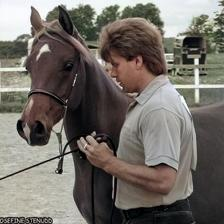
\includegraphics[scale=.4]{11_unet.jpeg}\\
            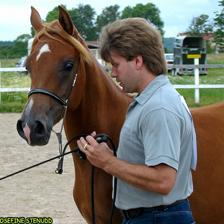
\includegraphics[scale=.4]{11_real.jpeg}
            \caption*{Cгенерированное U-Net и исходное изображения}
            %\label{fig:unet_example}
        \end{figure}
    \end{column}
\end{columns}
\end{frame}

\begin{frame}{План экспериментов}
%\framesubtitle{}
\begin{itemize}
    \item Модификация архитектуры \textbf{U-Net}: использование более сложных энкодеров, добавления улучшений, использованных в \textbf{DeOldify} (self-attention, spectral normalization).
    \item Обучение в режиме \textbf{NoGAN}. \textit{Опционально: решение проблемы автоматического поиска момента остановки обучения}.
    \item Эксперименты с loss-функцией, поиск оптимальных параметров для получения ярких изображений.
\end{itemize}
\end{frame}

\begin{frame}{Ссылки}
\begin{itemize}
    \item \href{https://github.com/vsgolovin/colorize/tree/Mailstone}{GitHub}
    \item \href{https://drive.google.com/drive/folders/1ebPVAsKlLlXY2Tg8Q1TXbiTRhfdegI40}{Google Drive}
\end{itemize}
\end{frame}

\end{document}